\documentclass{ximera}

%\documentclass{ximera}

\usepackage{float}
\usepackage{subcaption}

\pgfplotsset{compat=1.16}

\newtheorem{ass}{Assumption}

\def\check{\tikz\fill[scale=0.4](0,.35) -- (.25,0) -- (1,.7) -- (.25,.15) -- cycle;}





\outcome{We learn how our first options operate. Payoffs are explored. }

\author{Brad Waller}

%Section 2.1

\title{Calls and Puts}

\begin{document}

\begin{abstract}
We learn about our fundamental options. These will be revisited throughout much of the remainder of the book. Payoffs are of huge importance!
\end{abstract}

\maketitle

In our introductory chapter, we learned about some basic types of derivatives, namely forward contracts and futures arrangements. This chapter deals with a special type of derivative called an option. Options are contracts that are used to make trades based on some underlying asset.

\begin{definition}
A {\bf call option} gives the option owner the option to buy the underlying asset from the writer (seller) of the option. There are three things specified in the call option contract: the underlying asset, the time to expiration, and the {\bf strike price}. The strike price is the value that the owner would pay the writer in the event that the buyer exercises the option. A {\bf put option} gives the owner the option to sell the underlying asset to the writer of the option. That is the only difference between call options and put options. An options contract has no value after the expiration or the contract's exercise.
\end{definition}

There are two parties to options contracts: they buyer and the writer. The buyer is the position that we will usually consider, and it is the buyer that chooses to exercise the option. The writer is the individual that is willing to take a {\bf premium} at the time of sale to assume the liability of the options contract.

In addition to the characteristics in the definition, there is another component to an option. It is called {\bf style}. The style of the option dictates timing of exercise. In addition, it may influence the computation of the payoffs. The two styles we will focus on for now will be American and European. An American option that expires at time $T$ may be exercised at any time in the interval $(0,T]$. A European option with the same expiration may only be exercised at expiration. The additional opportunity to exercise provided by an American option gives it greater value than its European counterpart. In symbols, this would be
\begin{align*}
C_{am}\geq&C_{eu}\\
P_{am}\geq&P_{eu}
\end{align*}
where all other terms are assumed to be the same. 

In the above inequalities, I am using the symbols to denote values or prices of the options. These same symbols may be used to describe a specific portfolio. When variables between options are the same, they will be supressed. For example
\begin{equation*}
10c(30)+5c(40)-15c(50)
\end{equation*}
is the number that represents the value of the portfolio consisting of 10 calls with strike 30, 5 calls with strike 40, and 15 {\bf written} calls with strike 50. All of the options have the same underlying asset, time to expiration, and by default we will assume that they are European.

Let's examine the payoffs of some of our European options.

\begin{center}
	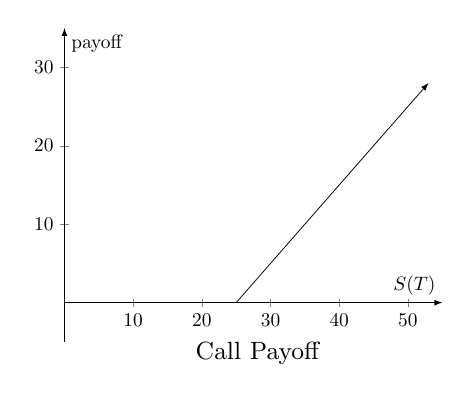
\begin{tikzpicture}[scale=0.7]
	\begin{axis}[
		xmin=0,
		xmax=55,
		%xtick={5,10,...,50},
		ymin=-5,
		ymax=35,
		%ytick={-20,-10,...,50},
		%grid=both,
		axis lines=middle,
		axis line style={->, >=latex},
		%x label style={at={(0.9,0.05)}},
		%x label style={at={(axis description cs:0.86,0.42)},anchor=north},
		xlabel={$S(T)$},
		ylabel={payoff}]
		%style={font=\tiny}]
		\addplot[black, smooth, domain=25:53, ->, >=latex]{x-25};
	\end{axis}
	\node at (3.5, -0.2){\small Call Payoff};
	\end{tikzpicture}
	\hspace{10pt}
	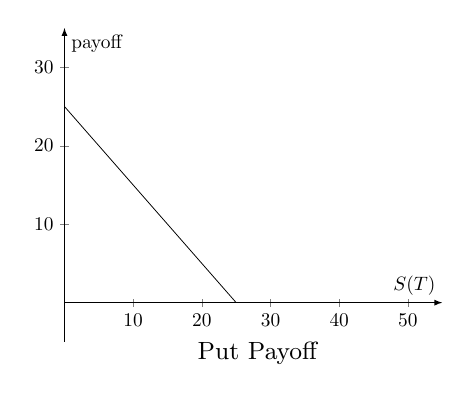
\begin{tikzpicture}[scale=0.7]
	\begin{axis}[
		xmin=0,
		xmax=55,
		%xtick={5,10,...,50},
		ymin=-5,
		ymax=35,
		%ytick={-20,-10,...,50},
		%grid=both,
		axis lines=middle,
		axis line style={->, >=latex},
		%x label style={at={(axis description cs:0.86,0.42)},anchor=north},
		xlabel={$S(T)$},
		ylabel={payoff}]
		%style={font=\tiny}]
		\addplot[black, smooth, domain=0:25, -, >=latex]{25-x};
	\end{axis}
	\node at (3.5, -0.2){\small Put Payoff};
	\end{tikzpicture}
\end{center}

Let's work through the reasoning attached to the diagram for the European call option with strike $25$ and expiration $T$. If you are the option holder, you have the choice to buy the underlying asset for $25$. If the market value is less than the strike value, would you buy at the strike price? Your answer should be no. If you wanted the asset, and the asset was valued less than the strike you would purchase it on the market. In this case, you allow the option to expire without exercise. In the event that the market price was greater than (or equal to) the strike price, you would exercise the option and purchase the asset for the strike price. You could then immediately sell the asset at the market price to receive the payoff of $S(T)-25$. The payoffs of our European options are
\begin{equation*}
\text{Time $T$ Call Payoff}=\max\{S(T)-K,0\}=
	\begin{cases}
	S(T)-K & \text{if } S(T)> K\\
	0&\text{otherwise,}
	\end{cases}
\end{equation*}
\begin{equation*}
\text{Time $T$ Put Payoff}=\max\{0,K-S(T)\}=
	\begin{cases}
	0 & \text{if }S(T)> K\\
	K-S(T)&\text{otherwise.}
	\end{cases}
\end{equation*}
Please work through reasoning used to determine the call's payoff in your determination of the put's payoff.

\begin{example}
Suppose that I buy 30 European call options on XYZ. The options all have strike $50$, and the options expire in one week. In one week, the price of one share of XYZ is 52.37. What is the payoff of my position in one week?
\end{example}

\begin{solution}
Since the price at expiration is greater than the strike, I would exercise the options. The payoff is
	\begin{equation*}
	30\cdot(52.37-50)=71.10
	\end{equation*}
\end{solution}

Why don't you try something more challenging. In the following, you will be purchasing and writing options. A written option has payoff that is $-1$ times the payoffs given above. We did something similar when we discussed the seller of a forward contract.

\begin{question}
You enter into several options contracts on the asset ZYX. They are all European, and they expire in one month. Your position follows.
	\begin{itemize}
	\item 50 calls with strike 40\\
	\item 20 calls with strike 45\\
	\item 70 written calls with strike 50\\
	\item 10 puts with strike 60
	\end{itemize}
At the end of the month, the share price of ZYX is $55$. What is your payoff?
	\begin{prompt}
		\begin{equation*}
		\text{Your payoff is}=\answer{650}
		\end{equation*}
	\end{prompt}
\end{question}

\begin{solution}
Strangely enough, each of the four options has a payoff! It is probably easiest to compute each as its own entity.
	\begin{align*}
	50\cdot\max\{55-40,0\}&=750\\
	20\cdot\max\{55-45,0\}&=200\\
	-70\cdot\max\{55-50,0\}&=-350\\
	10\cdot\max\{0, 60-55\}&=50
	\end{align*}
Summing the results yields 650. 
\end{solution}

As a ``fun'' exercise, let's try and graph the payoff of your position over all values! This may seem like it is a very difficult task, but there is something that should guide you in all of your work: all of the individual payoffs are piecewise linear (and continuous). The result of summing piecewise linear (and continuous) functions is also piecewise linear (and continuous). To determine how to draw the diagram, you only need to determine where the result will change slope.

 In our example, this occurs at the values $S(T)=40, 45, 50, \text{ and }60$. The payoffs are $200, 450, 700,$ and $600$, respectively. This gives us four points on our graph. We can connect the dots with a line, and we have the desired diagram; however, we still need to continue the diagram beyond $S(T)=60$ and before $S(T)=40$. For the former, we note that the slope must be 0. This is because the put does not contribute anything to the payoff for large values of $S(T)$. For the latter, the put is the only contributing factor. Since there are 10 puts, the slope will be $-10$. 

\begin{center}
	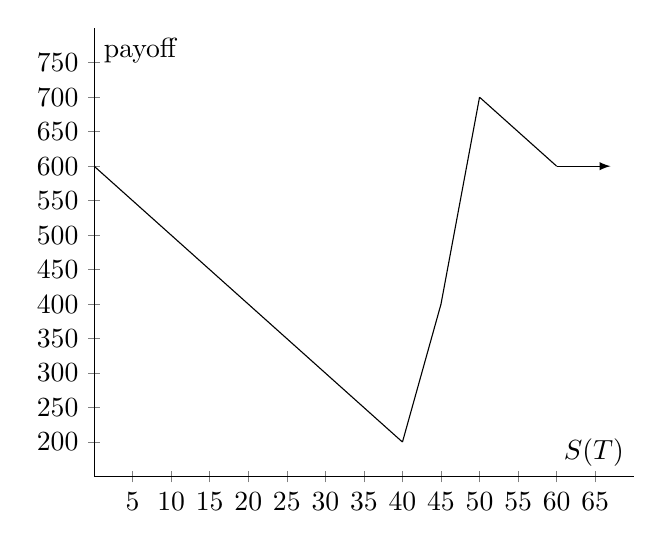
\begin{tikzpicture}
	\begin{axis}[
		xmin=0,
		xmax=70,
		xtick={5,10,..., 65},
		ymin=150,
		ymax=800,
		ytick={200,250,..., 750},
		%grid=both,
		axis lines=middle,
		axis line style={-, >=latex},
		%x label style={at={(1,1)}},
		%y label style={at={(-0.1,0.12)}, rotate=90},
		%y axis = {label={[node style={fill=blue!20}]{$x^2$}}},
		%{at={(axis description cs:0.86,0.42)},anchor=north},
		xlabel={$S(T)$},
		ylabel={payoff}]
		%style={font=\tiny}]
		\addplot[black, smooth, domain=0:40, -, >=latex]{-10*x+600};
		\addplot[black, smooth, domain=60:67, ->, >=latex]{600};
		\addplot[black, smooth, domain=50:60, -, >=latex]{-10*(x-50)+700};
		\addplot[black, smooth, domain=45:50, -, >=latex]{60*(x-45)+400};
		\addplot[black, smooth, domain=40:45, -, >=latex]{40*(x-40)+200};
	\end{axis}
	\end{tikzpicture}
\end{center}

In everything we've done so far in this section there has been no consideration to prices of the options. We will consider various models to determine prices of the options later in the course; however, it should be clear that they option buyer must pay something for the options. This is because they always have a positive payoff, and they never suffer any liability. It follows that the profit diagrams for the two types of European options will look like the image below.

\begin{center}
	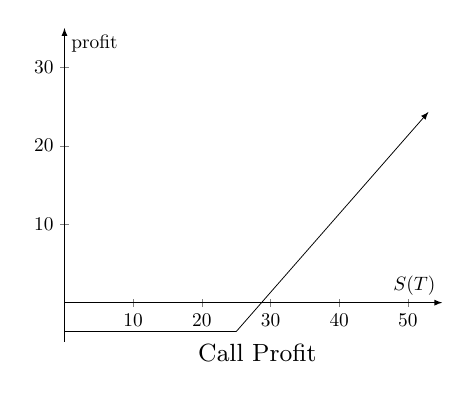
\begin{tikzpicture}[scale=0.7]
	\begin{axis}[
		xmin=0,
		xmax=55,
		%xtick={5,10,...,50},
		ymin=-5,
		ymax=35,
		%ytick={-20,-10,...,50},
		%grid=both,
		axis lines=middle,
		axis line style={->, >=latex},
		%x label style={at={(0.9,0.05)}},
		%x label style={at={(axis description cs:0.86,0.42)},anchor=north},
		xlabel={$S(T)$},
		ylabel={profit}]
		%style={font=\tiny}
		\addplot[black, smooth, domain=25:53, ->, >=latex]{x-25-3.69};
		\addplot[black, smooth, domain=0:25, -, >=latex]{-3.69};
	\end{axis}
	\node at (3.5, -0.2){\small Call Profit};
	\end{tikzpicture}
	\hspace{10pt}
	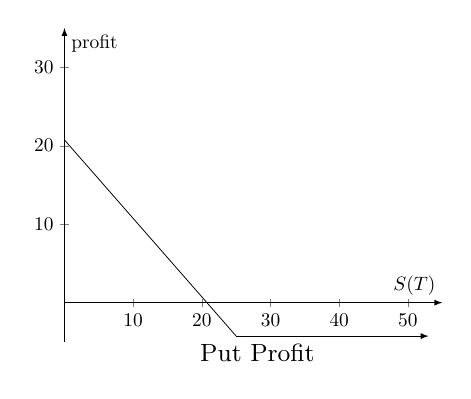
\begin{tikzpicture}[scale=0.7]
	\begin{axis}[
		xmin=0,
		xmax=55,
		%xtick={5,10,...,50},
		ymin=-5,
		ymax=35,
		%ytick={-20,-10,...,50},
		%grid=both,
		axis lines=middle,
		axis line style={->, >=latex},
		%x label style={at={(axis description cs:0.86,0.42)},anchor=north},
		xlabel={$S(T)$},
		ylabel={profit}]
		%style={font=\tiny}]
		\addplot[black, smooth, domain=0:25, -, >=latex]{25-x-4.26};
		\addplot[black, smooth, domain=25:53, ->, >=latex]{-4.26};
	\end{axis}
	\node at (3.5, -0.2){\small Put Profit};
	\end{tikzpicture}
\end{center}

It is natural to wonder why anybody would want an options contract. There are many reasons. 
\begin{itemize}
\item If you currently own shares of a company's stock, and you would like to protect your investment from losses in its value, you could purchase put options. This allows you to pick a price today to sell your asset to another party in the future. 
\item If you are currently the short seller in some asset, you could purchase calls using some of the proceeds of your short sale. These call options would lock in a maximum price that you could buy back the asset when you close out your short sale.
\item You could write calls on an asset that you own. This can be viewed as a way to enhance an investment's rate of return, provided you are comfortable with selling the asset to the buyer of the option at expiration if the asset price is greater than the strike price. This strategy is not advised if you are unwilling to part with the underlying asset.
\item You could enter into the options market as a speculator, wishing only to trade the options themselves with no interest in the underlying asset. This can be very lucrative since many options are quite elastic! More on elasticity will be seen in later chapters.
\end{itemize}

The first two items would be considered hedging strategies because they protect you from negative moves in the asset's value.

\begin{remark}
Many types of insurance may be viewed as options contracts. For example, if you buy a homeowner's policy that covers damages on your home in excess of \$5000 and your home is destroyed, then the policy will pay you the value of your home minus \$5000. This would be similar to an American put option on your home with strike \$5000 because they payoffs to you are identical. It is for this reason that actuaries are interested in options.
\end{remark}

Let's see an example of one of the hedging strategies.

\begin{example}
Suppose that you short sell 100 shares of ZYX. You have the following information:
	\begin{itemize}
	\item $S(0)=50$,
	\item $\delta=0.03$,
	\item $p=0.8$
	\item $m=0.01$, and
	\item $r=0.07$.
	\end{itemize}
In addition, you hedge your position by purchasing 101.51 European call options with strike 50 that all expire in six months. What is the profit of your porition if $S(0.5)=65$ if the price of the calls was \$469.52?
\end{example}

\begin{solution}
We have seen this example previously, and the profit without the calls was $-\$1542.57$. The computation is altered now. We will proceed in two ways:
	\begin{enumerate}
	\item we will view the portfolio as its parts, or
	\item we will view the portfolio as a whole.	
	\end{enumerate}
Both should yield the same result.

The profit of the call options is a straight-forward computation, as the payoff is obviously\\
$101.51(65-50)=1522.65$.
	\begin{equation*}
	1522.65-469.52e^{0.07\cdot 0.5}=1036.41
	\end{equation*}
It follows that the profit of the whole position is the sum of the parts:\\
 $-1542.57+1036.41=-\$506.16$

We won't always have the benefit of knowing the short sale's profit. Let's see the second approach. Recall that the short sale requires 80\% collateral. Our setup would look something like this where the payoff is in the first set of parenthesis and the profit is the negative at the end of the equation.
	\begin{equation*}
	100\left(S(0)e^{0.07\cdot 0.5}+0.8S(0)e^{0.01\cdot 0.5}-S(0.5)e^{0.03\cdot 0.5}+[S(0.5)-50]e^{0.03\cdot 0.5}\right)-469.52e^{0.07\cdot 0.5}
	\end{equation*}
Now, before doing too much, notice that we could change the equation as follows:
	\begin{equation*}
	100\left(S(0)e^{0.07\cdot 0.5}+0.8S(0)e^{0.01\cdot 0.5}-50e^{0.03\cdot 0.5}\right)-469.52e^{0.07\cdot 0.5}
	\end{equation*}
It's as though we altered the short-sale payoff by changing $S(0.5)$ to 50. That is the benfit of having the call options. The reason this is permitted is because the quantity of call options is the same as the quantity of shares at the time of the buyback. The value of the last equation is $-\$506.14$. We can attribute the difference to some rounding error. The benefit of the second approach is that it allows you to view the portfolio as a modified short sale. That can save you time when dealing with complex portfolios.

It should be clear that our poortfolio benefited from the purchase of the call options. Try graphing the profit of this position for various values of the underlying asset at expiration. After graphing the profit, it should be clear that there is a trade off taking place. Think about what that might be.
\end{solution}



\end{document}

